% -*- TeX -*-
\documentclass[aspectratio=169]{beamer}
\usepackage{booktabs}
\usepackage[edges]{forest}

\title{PyLith v3.0 Tutorial}
\subtitle{CIG and PyLith Best Practices}
\author{Brad Aagaard \\
  Charles Williams \\  
  Matthew Knepley}
\institute{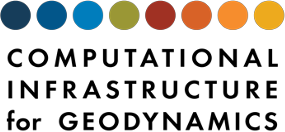
\includegraphics[scale=1.5]{../../logos/cig_logo_dots}%
  \hspace{4em}%
\raisebox{1em}{\includegraphics[scale=1.0]{../../logos/cig_short_pylith}}}
\date{June 21, 2022}


% ---------------------------------------------------- CUSTOMIZATION
\usetheme{CIG}
% Style information for PyLith presentations.

% Colors
\definecolor{ltorange}{rgb}{1.0, 0.74, 0.41} % 255/188/105
\definecolor{orange}{rgb}{0.96, 0.50, 0.0} % 246/127/0

\definecolor{ltred}{rgb}{1.0, 0.25, 0.25} % 255/64/64
\definecolor{red}{rgb}{0.79, 0.00, 0.01} % 201/0/3

\definecolor{ltpurple}{rgb}{0.81, 0.57, 1.00} % 206/145/255
\definecolor{purple}{rgb}{0.38, 0.00, 0.68} % 97/1/175

\definecolor{ltblue}{rgb}{0.2, 0.73, 1.0} % 51/187/255
\definecolor{mdblue}{rgb}{0.28, 0.50, 0.80} % 72/128/205
\definecolor{blue}{rgb}{0.12, 0.43, 0.59} % 30/110/150

\definecolor{ltltgreen}{rgb}{0.7, 1.00, 0.7} % 96/204/14
\definecolor{ltgreen}{rgb}{0.37, 0.80, 0.05} % 96/204/14
\definecolor{green}{rgb}{0.23, 0.49, 0.03} % 59/125/8
  
\definecolor{dkslate}{rgb}{0.18, 0.21, 0.28} % 47/53/72
\definecolor{mdslate}{rgb}{0.45, 0.50, 0.68} % 114/127/173
\definecolor{ltslate}{rgb}{0.85, 0.88, 0.95} % 216/225/229


\newcommand{\includefigure}[2][]{{\centering\includegraphics[#1]{#2}\par}}
\newcommand{\highlight}[1]{{\bf\usebeamercolor[fg]{structure}#1}}
\newcommand{\important}[1]{{\color{red}#1}}
\newcommand{\issue}[2]{\item[Issue:] {\color{red}#1}\\{\item[Soln:] \color{blue}#2}\\[4pt]}

\setbeamercolor{alerted text}{fg=ltgreen}
\setbeamertemplate{description item}[align left]


\newcommand{\lhs}[1]{{\color{blue}#1}}
\newcommand{\rhs}[1]{{\color{red}#1}}
\newcommand{\annotateL}[2]{%
  {\color{blue}\underbrace{\color{blue}#1}_{\color{blue}\mathclap{#2}}}}
\newcommand{\annotateR}[2]{%
  {\color{red}\underbrace{\color{red}#1}_{\color{red}\mathclap{#2}}}}
\newcommand{\eqnannotate}[2]{%
  {\color{blue}%
  \underbrace{\color{black}#1}_{\color{blue}\mathclap{#2}}}}

\newcommand{\trialvec}[1][]{{\vec{\psi}_\mathit{trial}^{#1}}}
\newcommand{\trialscalar}[1][]{{\psi_\mathit{trial}^{#1}}}
\newcommand{\basisvec}[1][]{{\vec{\psi}_\mathit{basis}^{#1}}}
\newcommand{\basisscalar}[1][]{{\psi_\mathit{basis}^{#1}}}

\newcommand{\tensor}[1]{\bm{#1}}
\DeclareMathOperator{\Tr}{Tr}

\usefonttheme[onlymath]{serif}

% minted shortcuts
\newminted{cfg}{bgcolor=ltslate,autogobble,fontsize=\tiny}
\newminted{bash}{bgcolor=ltltgreen,autogobble,fontsize=\tiny}

% PyLith components
\newcommand{\pylith}[1]{{\ttfamily\color{magenta}#1}}



% ========================================================= DOCUMENT
\begin{document}

% ------------------------------------------------------------ SLIDE
\maketitle

\logo{\includegraphics[height=4.5ex]{../../logos/cig_short_pylith}}


% ========================================================== SUBSECTION
\section{Introduction}

% ------------------------------------------------------------ SLIDE
\begin{frame}
  \frametitle{CIG Best Practices}
  \summary{\url{https://geodynamics.org/software/software-bp/}}
  
  \begin{itemize}
    \hitem{Software Development Best Practices}
    \begin{description}
    \item[Minimum] Minimum standards that all codes hosted by or distributed by CIG are expected to meet
    \item[Standard] Suite of standards CIG-supported codes should be following
    \item[Target] Desirable practices that developers should consider in defining long-term development priorities for codes developed within the CIG community
    \end{description}
    \hitem{Training Best Practices}\\
    Best practices for tutorials and hackathons for training users.
  \end{itemize}
      
\end{frame}


% ------------------------------------------------------------ SLIDE
\begin{frame}[t]
  \frametitle{CIG Software Development Best Practices}
  \summary{\url{https://geodynamics.org/software/software-bp/}}

  \vspace*{-8pt}{\tiny
    \begin{tabular}{lp{3.2cm}p{3.2cm}p{3.2cm}}
      % \toprule
      & {\bfseries Minimum} & {\bfseries Standard} & {\bfseries Target} \\ \midrule
      {\bf Licensing} & Open source & Same as Minimum & Same as Minimum \\ \midrule
      {\bf Version Control} & All source in version control. & Differentiate b/t maintenance and new development. & Feature branches. Stable development branches.\\ \midrule
      {\bf Coding} & & (a) Specify parameters at run time. (b) Development plan. (c) Add features without modifying main branch. \ldots & Standard + Output of provenance information. Parallel access to inputs/outputs. Checkpointing. \ldots \\ \midrule
      {\bf Portability} & (a) Code builds on Unix-like machines with free tools. (b) Portable build system. & Minimum + Dependency checking. Portable configuration and building. \ldots & Standard + Configure without modifying files under version control. Multiple builds using same source. \ldots \\ \midrule
      {\bf Testing} & Code includes tests that verify it runs properly. Results of accuracy and/or performance benchmarks. & Code includes pass/fail tests that verify it runs properly. & Pass/fail unit testing. Verification of physics via Method of Manufactured Solutions. \\ \midrule
      {\bf Documentation} & Install instructions. Description of parameters. Explanation of physics. Examples with input files. \ldots & Description of workflow for research use. Description of how to extend code in anticipated ways. & Standard + Guidelines on parameter ranges for which code is designed. FAQs or knowledge base. \\ \midrule
      {\bf User workflow} & & Change simulation parameters w/o rebuilding. User-specified directories and filenames for I/O. Use of standard binary formats. \ldots & Standard + Reproducibility via archiving of workflow. \\ %\bottomrule
    \end{tabular}}

\end{frame}


% ------------------------------------------------------------ SLIDE
\begin{frame}
  \frametitle{PyLith Best Practices}
  \summary{}

  PyLith development has strived to follow modern software development practices since its inception.

  \vfill
  \begin{itemize}
  \item Portable
  \item Modular
  \item Extensible
  \item Accessible to beginner users; don't impede advanced users
  \end{itemize}

\end{frame}


% ------------------------------------------------------------ SLIDE
\begin{frame}[t]
  \frametitle{PyLith Best Practices}
  \summary{}

  PyLith follows almost all CIG Standard and Target best practices
  \begin{itemize}
    \hitem{Git workflow} \only<2>{(see \href{https://pylith.readthedocs.io/en/latest/developer/contributing/workflow.html}{PyLith Developer Manual})}
    \begin{onlyenv}<2>
      \begin{itemize}
      \item Differentiate between maintenance and new development
      \item All changes are added in branches and merged using Pull Requests
      \item All Pull Requests must pass automated tests before being merged
      \end{itemize}
    \end{onlyenv}
    \hitem{Testing}
    \begin{onlyenv}<3>
      \begin{itemize}
      \item Unit tests at function level
      \item Method of Manufactured Solutions to verify implementation of physics
      \item Full-scale tests
      \item Benchmarks
      \end{itemize}
    \end{onlyenv}
    \hitem{Portability}
    \begin{onlyenv}<4>
      \begin{itemize}
      \item Binaries for macOS and Linux
      \item Runs on laptops to large clusters
      \item PyLith Installer utility for building from source on clusters
      \item Docker development environment
      \end{itemize}
    \end{onlyenv}
    \hitem{Development Plan} \url{}
    \begin{onlyenv}<5>
      \begin{itemize}
      \item Open collaboration with community to identify priorities
      \item Continuously evaluating priorities
      \end{itemize}
    \end{onlyenv}
  \end{itemize}

\end{frame}


% ------------------------------------------------------------ SLIDE
\begin{frame}[t]
  \frametitle{Ideas to consider}
  \summary{}


  \begin{itemize}
    \hitem{Use Git in your projects}
    \begin{onlyenv}<2>
      \begin{itemize}
      \item Reproducibility!
      \item Infinite undo
      \item Document changes to files
      \item Synchronize files across multiple computers with cloud storage
      \item Synchronize files with collaborators
      \item Experiment with an idea in a branch
      \end{itemize}
    \end{onlyenv}
    \hitem{Use an Integrated Development Environment}
    \begin{onlyenv}<3>
      \begin{itemize}
      \item Syntax highlighting for programming languages (includes brace matching)
      \item Git integration
      \item Linting (realtime syntax checking)
      \item Sophisticated editing
      \item Search and replace across project
      \item Interactive remote collaborative editing (files and terminals)
      \item Docker and SSH integration
      \end{itemize}
    \end{onlyenv}
  \end{itemize}

\end{frame}


% ------------------------------------------------------------ SLIDE
\begin{frame}[fragile]
  \frametitle{Example Git repository layout}
  \summary{GitLab and GitHub offer free, private repositories}

\begin{forest}
  file/.style = {text=orange},
  for tree={%
    folder,
    font=\scriptsize,
    text=blue,
    grow'=0,
    s sep=0,
    inner sep=1pt,
    outer sep=1pt,
    fit=band,
  }
  [projects/2019-ridgecrest
    [README.md, file]
    [modeling
      [README.md, file]
      [generate\_gmsh.py, file]
      [pylithapp.cfg, file]
      [coseismic.cfg, file]
      [postseismic.cfg, file]
      [utils]
      [viz]
      [input (not in repository)]
      [output (not in repository)]
      [scratch (not in repository)]
    ]
    [papers
      [2022-jgr]
    ]
    [presentations
      [2021-agu]
      [2022-ssa]
    ]
  ]  
\end{forest}  
%\includegraphics[height=6.0cm]{figs/repostructure}
  
\end{frame}


% ------------------------------------------------------------ SLIDE
\begin{frame}
  \frametitle{Integrated Development Environment (IDE)}
  \summary{}

  \begin{itemize}
    \hitem{Consider an IDE that supports a wide variety of programming languages}
    \begin{itemize}
    \item {\ttfamily Python}
    \item {\ttfamily cfg}
    \item {\ttfamily Markdown}
    \item {\ttfamily LaTeX}
    \end{itemize}
    \hitem{Examples}
    \begin{itemize}
    \item Visual Studio Code
    \item Atom
    \item Eclipse\\
      \noindent\vdots
    \end{itemize}
  \end{itemize}
  
\end{frame}


% ------------------------------------------------------------ SLIDE
\begin{frame}[t]
  \frametitle{PyLith Development Plan}
  \summary{}

  \begin{itemize}
    \hitem{Physics}
    \begin{onlyenv}<2>
      \begin{enumerate}
      \item Dynamic prescribed slip
      \item Spontaneous rupture (fault friction)
      \item Coupling quasi-static and dynamic problems for earthquake cycle modeling
      \item Poroelasticity and faulting
      \end{enumerate}
    \end{onlyenv}
    \hitem{Numerical}
    \begin{onlyenv}<3>
      \begin{enumerate}
      \item Parallel mesh loading
      \item Adaptive mesh refinement
      \item Adjoints for Bayesian inversion
      \end{enumerate}
    \end{onlyenv}
    \hitem{Maintainability}
    \begin{onlyenv}<4>
      \begin{enumerate}
      \item Pyre 1.X
      \item Convert examples to Jupyter notebooks
      \item Switch from SWIG to pybind11
      \item Add ability to chain together point-wise functions
      \end{enumerate}
    \end{onlyenv}
  \end{itemize}
  
\end{frame}

% ======================================================================
\end{document}


% End of file
